

\lstdefinelanguage{JavaScript}{
  keywords={typeof, new, true, false, catch, function, return, null, catch, switch, var, if, in, while, do, else, case, break},
  keywordstyle=\color{blue}\bfseries,
  ndkeywords={class, export, boolean, throw, implements, import, this},
  ndkeywordstyle=\color{darkgray}\bfseries,
  identifierstyle=\color{black},
  sensitive=false,
  comment=[l]{//},
  morecomment=[s]{/*}{*/},
  commentstyle=\color{purple}\ttfamily,
  stringstyle=\color{red}\ttfamily,
  morestring=[b]',
  morestring=[b]"
}


\lstset{
   language=JavaScript,
   backgroundcolor=\color{lightgray},
   extendedchars=true,
   basicstyle=\footnotesize\ttfamily,
   showstringspaces=false,
   showspaces=false,
   numbers=left,
   numberstyle=\footnotesize,
   numbersep=9pt,
   tabsize=2,
   breaklines=true,
   showtabs=false,
   captionpos=b
}


Colin comes with a Javascript engine. This engine gives access to the core features of colin, such as manipulation of structues. There will be access to more features, such as access to GUI elements in the feautre. We are still waiting with the implementation of those due to missing knowledge of what will be needed and in wich way it will be need. This means that the Javascript API will be exapanded in the next few releases. Of course we will try to fit it to your need - contact us!


\section{Debugger}

\section{Global}

These are the global objects present in the javscript engine you should know about:

\begin{trivlist}
	\leftskip=1cm
	\item[]\textbf{\texttt{print}} Function used for output, print(x) will print the value of x to the console.
	\item[]\textbf{\texttt{Math}} Contains matematical functions and constans, see section \ref{sec:jsMath}.
	\item[]\textbf{\texttt{ColinNode}} Prototype for nodes, see section \ref{sec:jsColinNode}.
	\item[]\textbf{\texttt{ColinBeam}} Prototype for beams, see section \ref{sec:jsColinBeam}.
	\item[]\textbf{\texttt{ColinLoad}} Prototype for loads, see section \ref{sec:jsColinLoad}.
	\item[]\textbf{\texttt{ColinBLS}} Prototype for BLS, see section \ref{sec:jsColinBLS}.
	\item[]\textbf{\texttt{ColinCLS}} Prototype for CLS, see section \ref{sec:jsColinCLS}.
	\item[]\textbf{\texttt{ColinSupport}} Prototype for supports, see section \ref{sec:jsColinSupport}.
	\item[]\textbf{\texttt{files}} Organisation of files, see section \ref{sec:jsFiles}.
	\item[]\textbf{\texttt{struct}} The current ColinStruct \ref{sec:jsColinStruct}}.
\end{trivlist}

\section{Files}
\label{sec:jsFiles}

You can access files using the \textbf{\texttt{files}} object.\\
Functions:

\begin{trivlist}
	\item[]\textbf{file information}
	\begin{trivlist}
		\leftskip=1cm
		\item[]\textbf{\texttt{int currentIndex()}}\\ Returns the index of the file you are currently editing.
		\item[]\textbf{\texttt{string filename(int i)}}\\ Returns the filename of file at index \texttt{i}.
		\item[]\textbf{\texttt{string filepath(int i)}}\\ Returns the absolute filepath of file at index \texttt{i}.
		\item[]\textbf{\texttt{int fileCount()}}\\ Returns the number of opened files.
		\item[]\textbf{\texttt{int tabCount()}}\\ Returns the number of active tabs which also contains the \texttt{settingspage} and the \texttt{starterpage}.
		\item[]\textbf{\texttt{void closeFile(int i)}}\\ Closes the file at index \texttt{i};
	\end{trivlist}
	\item[]\textbf{open and save}
	\begin{trivlist}
		\leftskip=1cm
		\item[]\textbf{\texttt{bool openT(string filename)}}\\ Open the file "\texttt{filename}". Returns \texttt{true} on success.
		\item[]\textbf{\texttt{bool saveAs(int i, string filename)}}\\ Saves the file number \texttt{i} as "\texttt{filename}". Returns \texttt{true} on success.
		\item[]\textbf{\texttt{bool save(int i)}}\\ Saves the file number \texttt{i}. Shows the save file dialog if no filename has been assigned to it yet. Returns \texttt{true} on success.
		\item[]\textbf{\texttt{bool saveCurrent(string filename)}}\\ Saves the file you are currently editing as "\texttt{fileName}". Returns \texttt{true} on success.
		\item[]\textbf{\texttt{bool saveCurrent()}}\\ Saves the file you are currently editiung. Shows the save file dialog if no filename has been assigned to it yet. Returns \texttt{true} on success.
	\end{trivlist}
	\item[]\textbf{starterpage and settingspage}
	\begin{trivlist}
		\leftskip=1cm
		\item[]\textbf{\texttt{void showNew()}}\\ Shows the \textit{starterpage}.
		\item[]\textbf{\texttt{void hideNew()}}\\ Hides the \textit{starterpage} if shown.

		\item[]\textbf{\texttt{void showSettings()}}\\ Shows the \textit{settingPage}.
		\item[]\textbf{\texttt{void saveSettings()}}\\ Saves all settings. Will be done on exit automatically.
		\item[]\textbf{\texttt{void closeSettings()}}\\ Closes the \textit{settingspage} if shown.
	\end{trivlist}
	\item[]\textbf{tabs}
	\begin{trivlist}
		\leftskip=1cm
		\item[]\textbf{\texttt{void nextTab()}}\\ Switches to the next tab. This does not only include opened files but also the \textit{starterpage} and \textit{settingspage}.
		\item[]\textbf{\texttt{void previousTab()}}\\ Switches to the previous tab. 
		\item[]\textbf{\texttt{void changeCurrentTo(int i)}}\\ Show the file number \texttt{i}.
	\end{trivlist}
\end{trivlist}

\section{ColinStruct}
\label{sec:jsColinStruct}

\begin{trivlist}
	\item[]\textbf{Managing Scripts}
	\begin{trivlist}
		\leftskip=1cm
		\item[] \texttt{void beginS(stirng name)}\\ Call this function before any other action if you want to merge more commands into one in the undo/redo history. Call \texttt{endS()} when you are done. The string \texttt{name} contains the name the command will have in the undo/redo history.
		\item[] \texttt{void endS()} \\Call this function to finish any merge. Don't forget to call this function or you will mess up the undo/redo functionality! If you are not shure, that your code runs without errors, you should put it in a try statement and make sure the script is always finished in the finally block: \\
		\texttt{try\{\dots your code \dots\}catch(e)\{\dots handle exception \dots\}finally\{endS()\}}.
	\end{trivlist}
	\item[]\textbf{Calculation}
	\begin{trivlist}
		\leftskip=1cm
		\item[]\textbf{\texttt{bool calculated}}\\ Property: Is true if forces and displacement of the structure has been calculated.
	\end{trivlist}
	\item[]\textbf{Nodes}
	\begin{trivlist}
		\leftskip = 1cm
		\item[] \textbf{\texttt{int nodeCount}}\\ Property: the number of nodes this structure contains. 
		\item[] \textbf{\texttt{ColinNode getNode(int i)}}\\ Function: Returns a copy of node number \texttt{i}.
		\item[] \textbf{\texttt{void setNode(int i, ColinNode n)}}\\ Function: Replaces the node number \texttt{i} of the file with the node \texttt{n}.
		\item[] \textbf{\texttt{int addNode(ColinNode n)}}\\ Function: Add the node \texttt{n} to the structure. Returns the index where it has been added.
		\item[] \textbf{\texttt{int addNode(double x, double z)}}\\ Function: Creates a new node with the coordinates (\texttt{x}, \texttt{z}) and adds it to the structure. Returns the index where the node has been added.
		\item[] \textbf{\texttt{void removeNode(int i)}}\\ Function: Removes the node at index \texttt{i}.
	\end{trivlist}
	\item[]\textbf{Supports} indirectly access through nodes is possible (\texttt{getNode(i).support})
	\begin{trivlist}
		\leftskip=1cm
		\item[] \texttt{void setSupport(int nodeIndex, ColinSupport s)}\\ Function: Replaces the support of node number \texttt{nodeIndex} with \texttt{s}.
		\item[] \texttt{void getSupport(int nodeIndex)}\\ Function: Returns a copy of the node at position \texttt{nodeIndex}.
	\end{trivlist}
	\item[]\textbf{Beams}
		\begin{trivlist}
		\leftskip = 1cm
		\item[] \textbf{\texttt{int beamCount}}\\ Property: the number of beams this structure contains. 
		\item[] \textbf{\texttt{ColinBeam getBeam(int i)}}\\ Function: Returns a copy of beam number \texttt{i}.
		\item[] \textbf{\texttt{void setBeam(int i, ColinBeam b)}}\\ Function: Replaces the beam number \texttt{i} of the file with the beam \texttt{b}.
		\item[] \textbf{\texttt{int addBeam(ColinBeam b)}}\\ Function: Add the beam \texttt{b} to the structure. Returns the index where it has been added.
		\item[] \textbf{\texttt{int addBeam(int leftN, int rightN)}}\\ Function: Creates a new beam with left node index \texttt{leftN} and right node index \texttt{rightN}. Material and cross section will be the same as the last beam added or the first material and cross section of the library. The new beam is added to the structure. It's index is the return value.
		\item[] \textbf{\texttt{void removeBeam(int i)}}\\ Function: Removes the beam at index \texttt{i}.
	\end{trivlist}
	\item[]\textbf{Loads}
		\begin{trivlist}
		\leftskip = 1cm
		\item[] \textbf{\texttt{int loadCount}}\\ Property: the number of loads this structure contains. 
		\item[] \textbf{\texttt{ColinLoad getLoad(int i)}}\\ Function: Returns a copy of load number \texttt{i}.
		\item[] \textbf{\texttt{void setLoad(int i, ColinLoad l)}}\\ Function: Replaces the load number \texttt{i} of the file with the load \texttt{l}.
		\item[] \textbf{\texttt{int addLoad(ColinLoad l)}}\\ Function: Add the load \texttt{l} to the structure. Returns the index where it has been added.
		\item[] \textbf{\texttt{void removeLoad(int i)}}\\ Function: Removes the load at index \texttt{i}.
	\end{trivlist}
	\item[]\textbf{BLS}
		\begin{trivlist}
		\leftskip = 1cm
		\item[] \textbf{\texttt{int blsCount}}\\ Property: the number of basic load sets this structure contains. 
		\item[] \textbf{\texttt{ColinBLS getBLS(int i)}}\\ Function: Returns a copy of the basic load set number \texttt{i}.
		\item[] \textbf{\texttt{void setBLS(int i, ColinBLS bls)}}\\ Function: Replaces the basic load set number \texttt{i} of the file with the basic load set \texttt{bls}.
		\item[] \textbf{\texttt{int addBLS(ColinBLS bls)}}\\ Function: Add the load set \texttt{bls} to the structure. Returns the index where it has been added. If you add a basic load set with a name already taken by another basic load set to the structure, a number will be appended to the name of the BLS.
		\item[] \textbf{\texttt{void removeBLS(int i)}}\\ Function: Removes the basic load set at index \texttt{i}.
	\end{trivlist}
	\item[]\textbf{CLS}
		\begin{trivlist}
		\leftskip = 1cm
		\item[] \textbf{\texttt{int clsCount}}\\ Property: the number of combined load sets this structure contains. 
		\item[] \textbf{\texttt{ColinCLS getCLS(int i)}}\\ Function: Returns a copy of the combined load set number \texttt{i}.
		\item[] \textbf{\texttt{void setCLS(int i, ColinCLS cls)}}\\ Function: Replaces the combined load set number \texttt{i} of the file with the combined load set \texttt{cls}.
		\item[] \textbf{\texttt{int addCLS(ColinCLS cls)}}\\ Function: Add the combined load set \texttt{cls} to the structure. Returns the index where it has been added. If you add a combined load set with a name already taken by another load set, a number will be appended to the name.
		\item[] \textbf{\texttt{void removeCLS(int i)}}\\ Function: Removes the combined load set at index \texttt{i}.
		\item[] \textbf{\texttt{void addBLStoCSL(int clsIndex, int blsIndex, double factor)}}: Function: Adds the basic load set at position \texttt{blsIndex} to the combined load set \texttt{clsIndex} multiplied by \texttt{factor}.
	\end{trivlist}
\end{trivlist}

\section{ColinNode}
\label{sec:jsColinNode}
\begin{trivlist}
	\item[] \textbf{Prototypes}
	\begin{trivlist}
		\leftskip=1cm
		\item[] \texttt{ColinNode()}\\ Prototype: Constructs a node with coordinates ()0,0);
		\item[] \texttt{ColinNode(double x, double z)}\\ Prototype: Constructs a node with coordinates (x,z).
	\end{trivlist}
	\item[] \textbf{Properties and Functions}
	\begin{trivlist}
		\leftskip=1cm
		\item[] \texttt{double x}\\ Property: the x coordinate of the node.\\ Unit: meter [m]
		\item[] \texttt{double z}\\ Property: the z coordinate of the node.\\ Unit: meter [m]
		\item[] \texttt{ColinSupprt support}\\ Property: the support of the node.
		\item[] \texttt{double angle}\\ Property: the angle of the node. \\ Unit: radiant [rad]
		\item[] \texttt{double[\ ] U}\\ Property: Array with the displacement in x direction for all combined load sets. At position \texttt{i} of the array you will find the result for the combined load set \texttt{i}.\\ Unit: meter [m]
		\item[] \texttt{double[\ ] W}\\ Property: Array with the displacement in z direction for all combined load sets. At position \texttt{i} of the array you will find the result for the combined load set \texttt{i}. \\ Unit: meter [m]
		\item[] \texttt{double[\ ] Phi}\\ Property: Array with the rotation of the node in deformed configuratipn for all combined load sets. At position \texttt{i} of the array you will find the result for the combined load set \texttt{i}.\\ Unit: radiant [rad]
		\item[] \texttt{double u} \\Property: Displacement in x direction. If you are using CLS this will be the result for the first CLS. \\ Unit: meter [m]
		\item[] \texttt{double w} \\Property: Displacement in z direction. If you are using CLS this will be the result for the first CLS. \\ Unit: meter [m]
		\item[] \texttt{double phi} \\Property: Rotation in deformed configuration. If you are using CLS this will be the result for the first CLS. \\ Unit: radiant [rad]
	\end{trivlist}
\end{trivlist}

\section{ColinBeam}
\label{sec:jsColinBeam}
\begin{trivlist}
	\item[]\textbf{Prototypes}
	\begin{trivlist}
		\leftskip=1cm
		\item[] \texttt{ColinBeam()}\\ Prototype: Constructs a beam with boath nodes zero.
		\item[] \texttt{ColinBeam(int leftN, int rightN)}\\ Prototype: Constructs a beam with left node \texttt{leftN} and right node \texttt{rightN}.
	\end{trivlist}
	\item[] \textbf{Properties and Function}
	\begin{trivlist}
		\leftskip=1cm
		\item[] \texttt{int leftNode} \\Property: Index of the left node of the beam.
		\item[] \texttt{int rightNode} \\Property: Index of the right node of the beam.
		\item[] \texttt{double l} \\Property: The length of the beam. This value is calculated the time the beam is exported to JavaScript. This means, this value is not available if it has been created by prototype.\\ Unit: meter[m]
		\item[] \texttt{double angle} \\Property: The angle between the beam axis and the global x axis. This value is calculated the time the beam is exported to JavaScript. This means, this value is not available if it has been created by prototype.
		\item[] \texttt{int material} \\ Property: Index of the material of the beam.
		\item[] \texttt{int cross section} \\ Property: Index of the cross section of the beam.
		\item[] \texttt{bool[6] hinges} \\Property: Holds the hinges for this beam in the following order:
		\begin{trivlist}
			\leftskip=1cm
			\item[] \texttt{hinges[0]}: left, x-direction
			\item[] \texttt{hinges[1]}: left, z-direction
			\item[] \texttt{hinges[2]}: left, rotation
			\item[] \texttt{hinges[3]}: right, x-direction
			\item[] \texttt{hinges[4]}: right, z-direction
			\item[] \texttt{hinges[5]}: right, rotation
		\end{trivlist}
		\item[] \texttt{double[6] springs} \\Property: Holds the springs connecting the beams left or right nodes with the actual beam ends if there is a hinge. The order is the same as for \texttt{hinges}.\\ Unit: newton per meter $\left[\frac{N}{m}\right]$ for indizes 0, 1, 3, 4 and newton meter per radiant $\left[\frac{Nm}{rad}\right]$ for indizes 2, 5
		\item[] \texttt{double[\ ][\ ] Narg} \\Property: Holds the coefficents for the polynom which describes the normal force function of the beam. The first index is the index of the combined load set for which these are valid. The second index is the index of the coefficent in the polynom:\\
		\begin{center}$N_{\text{cls}}(x) &= \sum \text{Narg}[\text{cls}][i]\cdot x^i $\end{center}
		\item[] \texttt{double[\ ][\ ] Qarg} \\Property: Holds the coefficents for the polynom which describes the shear force function of the beam. Equivalent order and evaluation as for \texttt{Narg}.
		\item[] \texttt{double[\ ][\ ] Marg} \\Property: Holds the coefficents for the polynom which describes the moment function of the beam. Equivalent order  and evaluation as for \texttt{Narg}.
		\item[] \texttt{double[\ ][\ ] uarg} \\Property: Holds the coefficents for the polynom which describes the displacement in x direction of the beam. Equivalent order and evaluation as for \texttt{Narg}.
		\item[] \texttt{double[\ ][\ ] warg} \\Property: Holds the coefficents for the polynom which describes the displacement in z direction of the beam. Equivalent order  and evaluation as for \texttt{Narg}.
		\item[] \texttt{double[\ ][\ ] parg} \\Property: Holds the coefficents for the polynom which describes the rotation of the beam. Equivalent order and evaluation  as for \texttt{Narg}.
		\item[] \texttt{double N(int cls, double x)} \\Function: Evaluates the polynom for the \textbf{normal force N} for the beam and returns the result. Parameters are the index of the CLS \texttt{cls} for which you want the results and the position on the beam \texttt{x}. \\Unit: newton [N]
		\item[] \texttt{double N(double x)} \\Function: Same as above. Returns the result for the first CLS (\texttt{N(x) = N(0, x)}). If you are not using CLS, this is the only function.\\Unit: newton[N]
		\item[] \texttt{double Q(int cls, double x)} \\Function: Evaluates the polynom for the \textbf{shear force Q} for the beam and returns the result. Parameters are the index of the CLS \texttt{cls} for which you want the results and the position on the beam \texttt{x}. \\Unit: newton [N]
			\item[] \texttt{double Q(double x)} \\Function: Same as above. Returns the result for the first CLS (\texttt{Q(x) = Q(0, x)}). If you are not using CLS, this is the only function.\\Unit: newton[N]
		\item[] \texttt{double M(int cls, double x)} \\Function: Evaluates the polynom for the \textbf{moment M} for the beam and returns the result. Parameters are the index of the CLS \texttt{cls} for which you want the results and the position on the beam \texttt{x}. \\Unit: newton meter [Nm]
		\item[] \texttt{double M(double x)} \\Function: Same as above. Returns the result for the first CLS (\texttt{M(x) = M(0, x)}). If you are not using CLS, this is the only function.\\Unit: newton[Nm]
		\item[] \texttt{double u(int cls, double x)} \\Function: Evaluates the polynom for the \textbf{displacement in x direction} for the beam and returns the result. Parameters are the index of the CLS \texttt{cls} for which you want the results and the position on the beam \texttt{x}. \\Unit: meter [m]
		\item[] \texttt{double u(double x)} \\Function: Same as above. Returns the result for the first CLS (\texttt{u(x) = u(0, x)}). If you are not using CLS, this is the only function.\\Unit: meter [m]
		\item[] \texttt{double w(int cls, double x)} \\Function: Evaluates the polynom for the\textbf{displacement in z direction} for the beam and returns the result. Parameters are the index of the CLS \texttt{cls} for which you want the results and the position on the beam \texttt{x}. \\Unit: meter [m]
		\item[] \texttt{double w(double x)} \\Function: Same as above. Returns the result for the first CLS (\texttt{w(x) = w(0, x)}). If you are not using CLS, this is the only function.\\Unit: meter [m]
		\item[] \texttt{double phi(int cls, double x)} \\Function: Evaluates the polynom for the \textbf{rotation} for the beam and returns the result. Parameters are the index of the CLS \texttt{cls} for which you want the results and the position on the beam \texttt{x}. \\Unit: radiant [rad]
		\item[] \texttt{double phi(double x)} \\Function: Same as above. Returns the result for the first CLS (\texttt{phi(x) = phi(0, x)}). If you are not using CLS, this is the only function.\\Unit: radiant [rad]
	
\end{trivlist}


\section{ColinLoad}
\label{sec:jsColinLoad}

\begin{trivlist}
	\item[]\textbf{Prototypes}
	\begin{trivlist}
		\leftskip=1cm
		\item[] \texttt{ColinLoad()}\\Prototype: Constructs a nodal load with invalid position, and all values set to zero.
		\item[] \texttt{ColinLoad(int type, int position, double Px, double Pz, double M)}\\ Prototype: Constructs a load. The type depends on the integer \texttt{type} (See property type). The beam or node this load is placed on is set with \texttt{position}. \texttt{Px} and \texttt{Pz} describe the horizontal and vertical Values of the load in newton[N]. M describes the Moment of the Load. If a property is not required for the load to construct, such as \texttt{M} for distributed loads, it is ignored. To create temperature changes, set \texttt{Px} to T, to create temperature differences, set \texttt{Pz} to T (you must set the right type too).
		\item[] \texttt{ColinLoad(int type, int position, double Px, double Pz, double M, int set)}\\Prototype: Same as above, but you can choose a basic load set this load is assigned to!
	\end{trivlist}
	\item[]\textbf{Properties and Functions}
	\begin{trivlist}
		\leftskip=1cm
		\item[]\texttt{double x}\\Property: x value for the load. Depending on the type the following:
		\begin{trivlist}
			\leftskip=2cm
			\item[] nodal load and double load: horizontal load. Unit: newton [N]
			\item[] distributed load: horizontal load. Unit: newton per meter [Nm]
			\item[] temperatur change: temperature difference between current temperature and temperature while assembling. Unit: Kelvin[K]
			\item[] else it is unused.
		\end{trivlist}
		\item[]\texttt{double z}\\Property: z value for the load. Depending on the type the following:
		\begin{trivlist}
			\leftskip=2cm
			\item[] nodal load and double load: vertical load. Unit: newton [N]
			\item[] distributed load:vectical load. Unit: newton per meter $\left[\dfrac{N}{m}\right]$
			\item[] temperatur difference: temperature difference between upper and lower side of the cross section. Unit: Kelvin[K]
			\item[] else it is unused.
		\end{trivlist}
	\end{trivlist}
	\item[]\textbf{double m}\\Property: The moment. used by the two types moment and double load.\\Unit: newton meter [Nm]
	\item[]\texttt{int beam}\\Property: The index of the beam this load is placed on. Only defined for loads placed on a beam (distributed loads, temperatur loads, double loads).
	\item[]\texttt{int node}\\Property: The index of the node this load is placed on. Only defined for loads placed on a node (nodal load and moment).
	\item[]\texttt{int type}\\Property: Describes the type of the load:
	\begin{trivlist}
		\leftskip=1cm
		\item[]0: nodal load
		\item[]1: moment
		\item[]2: uniformly distributed load
		\item[]3: increasing linear load
		\item[]4: decreasing linear load
		\item[]5: temperature changes
		\item[]6: temperature difference
		\item[]7: double load, left side of the beam
		\item[]8: double load, right side of the beam
	\end{trivlist}
	\item[]\texttt{int set}\\Property: The index of the basic load set which contains this load. A negative value if it is not assigned to any set.
\end{trivlist}


\section{ColinBLS}
\label{sec:jsColinBLS}
\begin{trivlist}
\item[]\textbf{Prototypes}
	\begin{trivlist}
		\leftskip=1cm
		\item[] \texttt{ColinBLS()}\\Prototype: Constructs a basic load set with no name.
		\item[] \texttt{ColinBLS(string name)}\\Prototype: Constructs a basic load set named \texttt{name}.
	\end{trivlist}
\item[]\textbf{Properties and Functions}
	\begin{trivlist}
		\leftskip=1cm
		\item[] \texttt{string name}\\Property: The name of set.
	\end{trivlist}
\end{trivlist}

\section{ColinCLS}
\label{sec:jsColinCLS}
\item[]\textbf{Prototypes}
	\begin{trivlist}
		\leftskip=1cm
		\item[] \texttt{ColinCLS()}\\Prototype: Constructs a combined load set with no name.
		\item[] \texttt{ColinCLS(string name)}\\Prototype: Constructs a combined load set named \texttt{name}.
	\end{trivlist}
\item[]\textbf{Properties and Functions}
	\begin{trivlist}
		\leftskip=1cm
		\item[] \texttt{string name}\\Property: The name of set.
		\item[] \texttt{bool active}\\Property: Decides weather the CLS is shown or hidden. Set active to true to show!
		\item[] \texttt{object[\ ] children}\\Property: The children represent the combination for this CLS. Each of these objects contains two properties:
		\begin{trivlist}
			\leftskip=2cm
			\item[]\texttt{int bls}\\The index of the BLS
			\item[]\texttt{double factor}\\The factor by which all loads of the BLS are multiplied.
		\end{trivlist}
	\end{trivlist}
\end{trivlist}

\section{ColinSupport}
\label{sec:jsColinSupport}
\begin{trivlist}
\item[]\textbf{Prototypes}
	\begin{trivlist}
		\leftskip=1cm
		\item[] \texttt{ColinSupport())}\\Prototype: Constructs a void support (no degree of freedom locked).
		\item[] \texttt{ColinSupport(bool x, bool z, bool phi)}\\Prototype: Constructs a support. The tree parameters \texttt{x}, \texttt{z} and \texttt{phi} decide weather the proper degree of freedom is locked or not.
	\end{trivlist}
\item[]\textbf{Properties and Functions}
	\begin{trivlist}
		\leftskip=1cm
		\item[] \texttt{bool x}\\Property: Locks degree of freedom in x direction.
		\item[] \texttt{bool z}\\Property: Locks degree of freedom in z direction.
		\item[] \texttt{bool phi}\\Property: Locks degree of freedom for rotation.
		\item[] \texttt{double cx}\\Property: The spring constant for the spring in x direction. If this value is not zero, it will overwrite \texttt{x}.\\Unit: newton per meter $\left[\dfrac{N}{m}\right]$
		\item[] \texttt{double cz}\\Property: The spring constant for the spring in z direction. If this value is not zero, it will overwrite \texttt{z}.\\Unit: newton per meter $\left[\dfrac{N}{m}\right]$
		\item[] \texttt{double cphi}\\Property: The spring constant for the rotation spring. If this value is not zero, it will overwrite \texttt{phi}.\\Unit: newton meter per radiant $\left[\dfrac{Nm}{rad}\right]$
	\end{trivlist}
\end{trivlist}

\section{Examples}

This section contains a few examples which show how to use the JavaScript API and for what it can be used. I will represent some code in listings. I will refer to those listings using (listing)[line] or [line]. if the listing to which i refer when i'm continuing to refer to the same listing. For example (4.1)[1] refers to listing 4.1 line 1.

\subsection{Creating a structure}
This example shows how to create nodes, beams, loads and supports and how to add them to a structure. I will create an arc in this example. \Colin can not handle arcs by itself. A possible solution is to create an arc with a lot of small beams. Doing this manually is pretty annoying, but we can create such an arc very quickly with a small script.
\vspace{20}\\
\begin{minipage}[h]{\textwidth-8cm}
\paragraph{Merging changes}
First of all, we tell \Colin to merge all following changes into a single step for the undo/redo list. Our script will trigger a few hundred changes to the structure. We want to undo them in a single step (\ref{lst:structcreation})[2] which we call \textit{creating an arc!}. Please note that i am not using a try-catch-finally statement, which is kind of risky when you are not shure your script is running without any exception!\end{minipage}
\hfill
\begin{minipage}[h]{8cm}
\begin{figure}[H]
\begin{center}
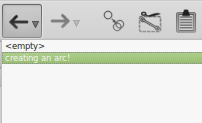
\includegraphics[width=\textwidth-2cm]{../pictures/scriptmerge.png}
\caption{merging scripts}
\label{pic:scriptmerge}
\end{center}
\end{figure}
\end{minipage}
\vspace{20pt}\\
\begin{minipage}[h]{\textwidth-8cm}
\paragraph{Creating nodes}
We start with the creation of nodes. We keep tracking which nodes we added. To do so we take a look at the number of nodes the structure contains before [1] we add any node and afterwards [5]. We use the function \texttt{addNode(double x, double z)} [3] to add nodes to our structure. An alternative would be to create a \texttt{ColinNode} object and pass it to the structure: \texttt{addNode(ColinNode(x, z))}. To add many nodes to our structure, we use a loop [2] and create an arc using \texttt{Math.sin(i)} and \texttt{Math.cos(i)} [3]. The interval for i of [0, $\pi$] leads to an arc of $180^\circ$ and a radius of one meter as shown in figure~\ref{pic:scriptnode}.
\end{minipage}
\hfill
\begin{minipage}[h]{8cm}
\begin{figure}[H]
\begin{center}
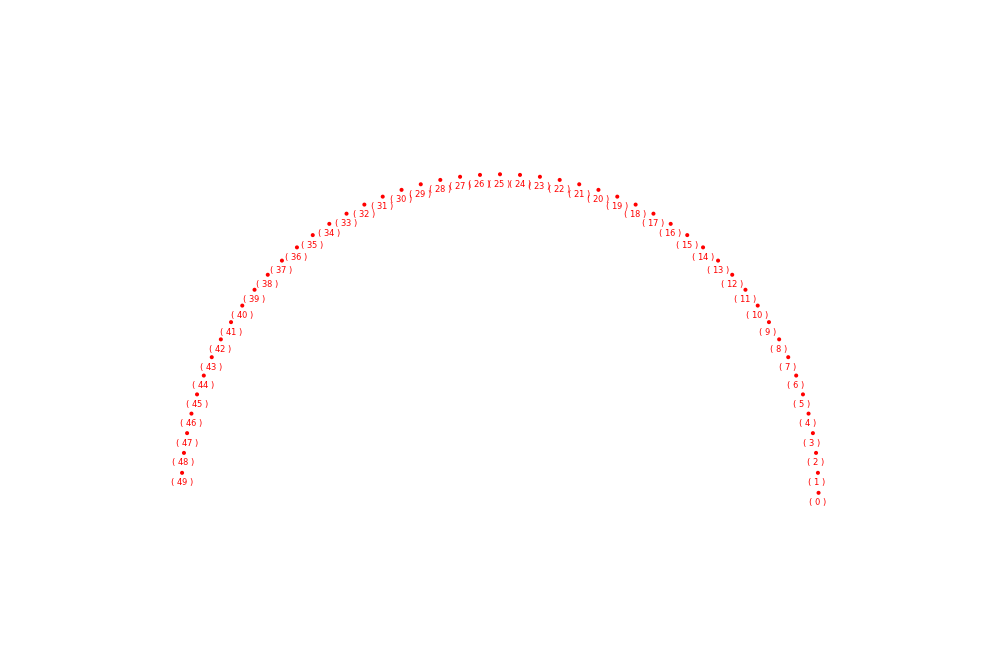
\includegraphics[width=\textwidth]{../pictures/scriptnode.png}
\caption{added nodes}
\label{pic:scriptnode}
\end{center}
\end{figure}
\end{minipage}
\vspace{20pt}\\
\begin{minipage}[h]{\textwidth-8cm}
\paragraph{Creating beams} The next step is to connect the created nodes with beams. We use a for loop once again [7] to add a beam which connects each node with the next one, beginning with the first node we added unit the last node we added. To create beams, we use the function \texttt{addBeam(int leftNode, int rightNode)} [8]. I will keep the interval of indices which mark the nodes we added with our script [6],[10]. As you can see in figure~\ref{pic:scriptbeam}, all our nodes are connected.
\end{minipage}
\hfill
\begin{minipage}[h]{8cm}
\begin{figure}[H]
\begin{center}
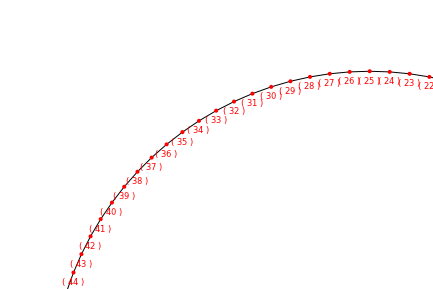
\includegraphics[width=\textwidth]{../pictures/scriptbeam.png}
\caption{added beams}
\label{pic:scriptbeam}
\end{center}
\end{figure}
\end{minipage}
\vspace{20pt}\\
\begin{minipage}[h]{\textwidth-8cm}
\paragraph{Creating supports} Now we set the supports. These will be placed at the two ends of our arc [11]-[12]. Once again we use \texttt{nodeBegin} and \texttt{nodeEnd} to identify our ends. We chose supports which lock the displacement but keep rotation possible by initializing new supports with \texttt{true, true, false}. You can see the change for one of the ends in figure~\ref{pic:scriptsupport}.
\end{minipage}
\hfill
\begin{minipage}[h]{8cm}
\begin{figure}[H]
\begin{center}
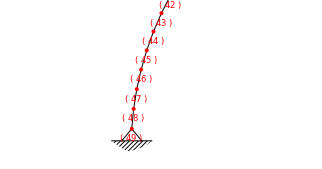
\includegraphics[width=\textwidth]{../pictures/scriptsupport.png}
\caption{added supports}
\label{pic:scriptsupport}
\end{center}
\end{figure}
\end{minipage}
\vspace{20pt}\\
\begin{minipage}[h]{\textwidth-8cm}
\paragraph{Creating loads} The next step is to add loads. In this example i will add a load to each beam, for which i use a loop [17]. Within the loop, i create a load with the prototype \texttt{ColinLoad(int type, int position, double Px, double Pz, double M)}[18]. In this example, a uniformly distributed load (\texttt{type = 2})), with a vectical load of $1\frac{kN}{m}$ will be created (\texttt{Pz = 1000}). The position is set by our counter for all beams \texttt{i}. After this step, your struct will look like in figure~\ref{pic:scriptload}
\end{minipage}
\hfill
\begin{minipage}[h]{8cm}
\begin{figure}[H]
\begin{center}
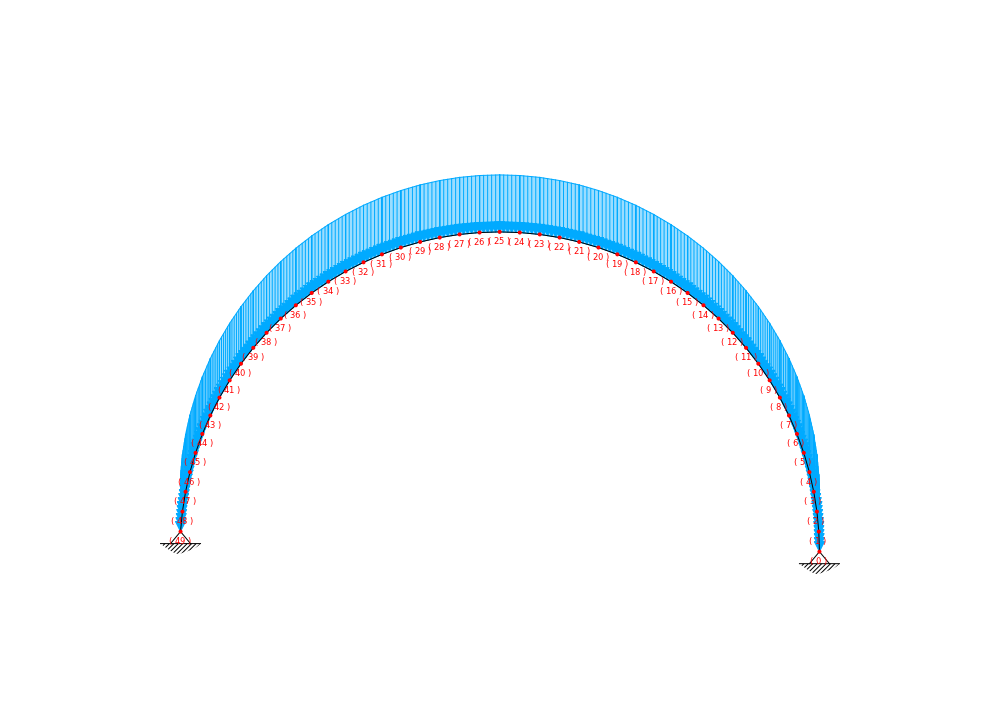
\includegraphics[width=\textwidth]{../pictures/scriptload.png}
\caption{added loads}
\label{pic:scriptload}
\end{center}
\end{figure}
\end{minipage}
\vspace{20pt}\\
We can now calculate the forces and the displacement of the structure we created, so i will stop with the fist example here. Figure~\ref{pic:scriptresult} shows the normal force in our arc! I will continuing with this structure in further examples! 
\begin{figure}[H]
\begin{center}
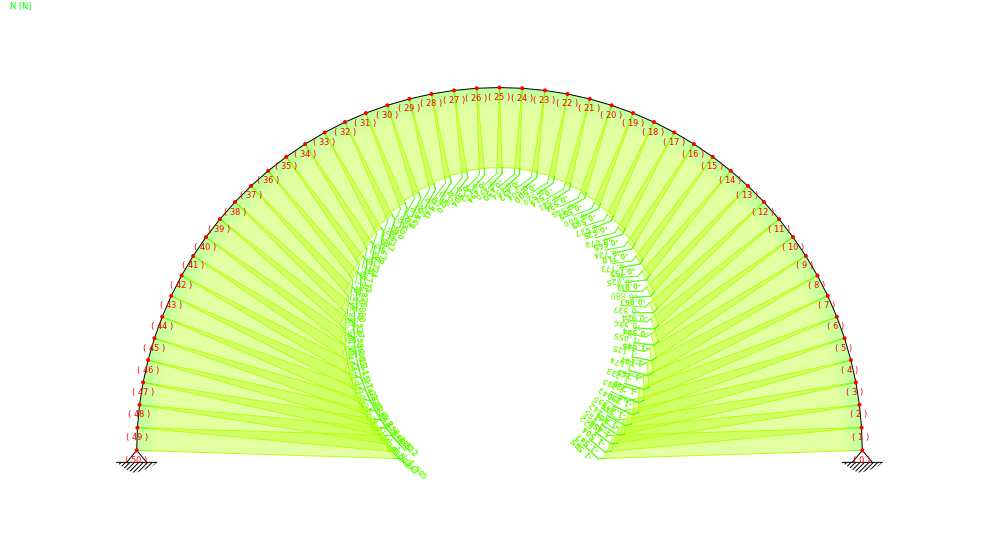
\includegraphics[width=\textwidth]{../pictures/scriptresult.png}
\caption{normal force in the arc}
\label{pic:scriptresult}
\end{center}
\end{figure}
\vspace{20pt}\\

\begin{lstlisting}[frame=single, basicstyle=\small, label=lst:structcreation, caption=creating a structure, numbers=left, firstnumber=1, tabsize=3]
//merge all commands to one
struct.beginS("creating an arc!");
//creating nodes
var nodeBegin = struct.nodeCount;
for(i=0; i<=Math.PI+0.01; i+=Math.PI/50){
	struct.addNode(Math.cos(i), -Math.sin(i));
}
var nodeEnd = struct.nodeCount-1;
//creating beams
var beamBegin = struct.beamCount;
for(i=nodeBegin+1; i<=nodeEnd; i++){
	struct.addBeam(i-1, i);
}
var beamEnd = struct.beamCount-1;
//creating supports
struct.setSupport(nodeBegin, ColinSupport(true, true, false));
struct.setSupport(nodeEnd, ColinSupport(true, true, false));
//creating loads
for(i=beamBegin; i<=beamEnd; i++){
	struct.addLoad(ColinLoad(2, i, 0, 1000, 0));
}
//end with merging commands
struct.endS();
\end{lstlisting}

\section{Adding load sets}

In this example i will show how to add basic load sets to the structure, and how to edit existing loads to assign them to basic load sets. Also, i will create some combined load sets!
\vspace{20pt}\\
\begin{minipage}[h]{\textwidth-8cm}
\paragraph{Creating load sets} First, i will create two basic load sets, called \textit{wind} and \textit{gravity} and some combined load sets, called \textit{wind}, \texit{gravity}, \textit{wind+gravity} and \textit{wind+gravity2}. As you can see in (\ref{lst:setcreation})[1]-[2] and [3]-[5], the syntax for both is the same, the function name is slightly different. Figure~\ref{pic:scriptset} shows the sets in the tree representation. The colors for the sets are black. You can set them in the treeview manually.
\end{minipage}
\hfill
\begin{minipage}[h]{8cm}
\begin{figure}[H]
\begin{center}
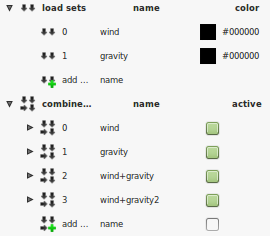
\includegraphics[width=\textwidth-1cm]{../pictures/scriptset.png}
\caption{added sets}
\label{pic:scriptset}
\end{center}
\end{figure}
\end{minipage}
\vspace{20pt}\\
\begin{minipage}[h]{\textwidth-8cm}
\paragraph{Assign existing loads} Your structure already contains loads. In the next step i will assign all those loads to our basic load set \textit{gravity}. We do this once for every load, which we can do with the for loop [8]. In the loop we get a copy of the load [9] and change it's set to 0 [10], which is the index of our basic load set \textit{gravity}. Afterwards we set the changed load to our structure [11]. As you can see at the color of the loads in figure~\ref{pic:scriptsetset}, all our loads are assigned to the load set with the color green (set the color of it manually).
\end{minipage}
\hfill
\begin{minipage}[h]{8cm}
\begin{figure}[H]
\begin{center}
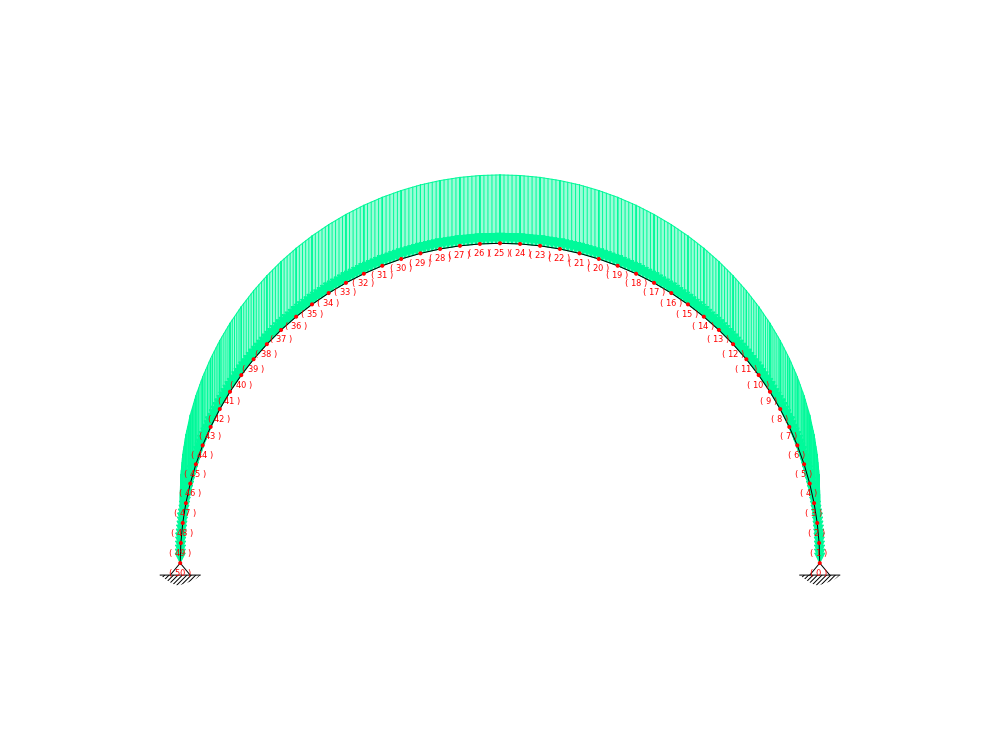
\includegraphics[width=\textwidth-1cm]{../pictures/scriptsetset.png}
\caption{assigned loads to sets}
\label{pic:scriptsetset}
\end{center}
\end{figure}
\end{minipage}
\vspace{20pt}\\
\begin{minipage}[h]{\textwidth-8cm}
\paragraph{Create new loads} Now we will create new loads and assign them directly to our basic load set \textit{wind}. As an example for a load caused by wind, i will create loads normal to the beam they are placed on.
\end{minipage}
\hfill
\begin{minipage}[h]{8cm}
\begin{figure}[H]
\begin{center}
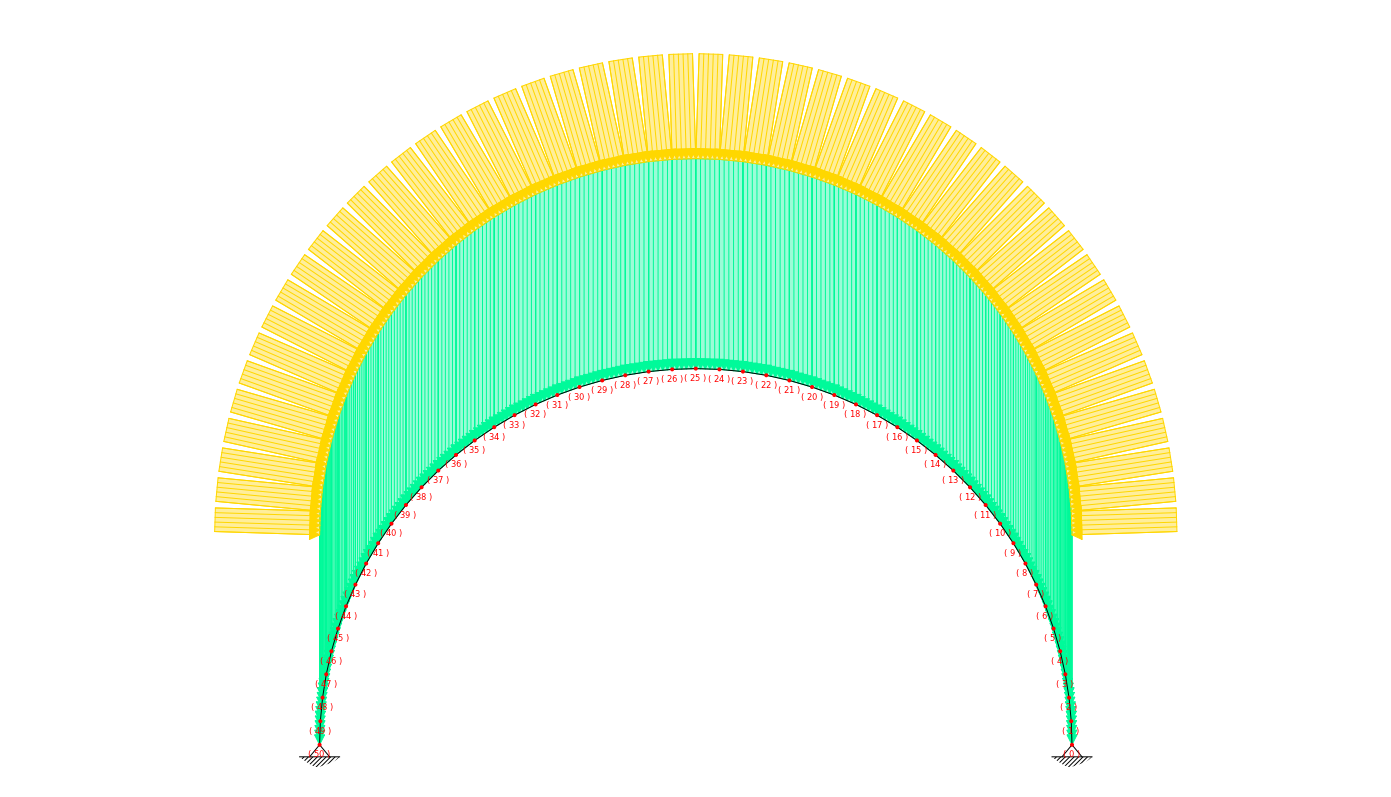
\includegraphics[width=\textwidth-1cm]{../pictures/scriptmoreload.png}
\caption{adding more loads}
\label{pic:scriptmoreload}
\end{center}
\end{figure}
\end{minipage}
\vspace{20pt}\\
\begin{minipage}[h]{\textwidth-8cm}
\paragraph{Combine load sets} In the last step we want to create combinations of your basic load sets. In line [16] and [17] i add the first BLS to the first CLS and the second BLS to the second BLS using a function of the structure \texttt{void addBLStoCLS(cls, bls, factor)}.\\
In line [20]-[28] i create a combination of the two basic load sets \texit{wind} and \textit{gravity} and put them into the CLS \text{wind+gravity}. This time i use another way to create them. First i get a copy of the proper CLS [20]. Then i initialize the children of this CLS to an array with length two [21]. Afterwards i create an object [22] and set it's parameter \texttt{bls} [23] and \texttt{fac} [24] to the designated values. I repeat the same for the BLS with index 1. Afterwards i return the changed CLS to the structure in line [28]. I do the same with CLS at index 3 with some modified factors.
\end{minipage}
\hfill
\begin{minipage}[h]{8cm}
\begin{figure}[H]
\begin{center}
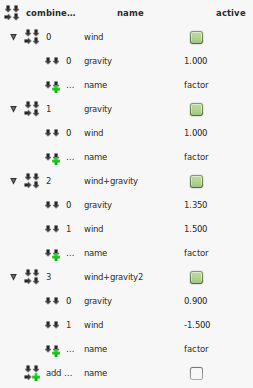
\includegraphics[width=\textwidth-1cm]{../pictures/scriptclscreated.png}
\caption{created the CLS}
\label{pic:scriptclscreated}
\end{center}
\end{figure}
\end{minipage}\\

We have now created four combinations of two sets. The results can be seen in figure~\ref{pic:scriptclsfinished}.
\begin{figure}[H]
\begin{center}
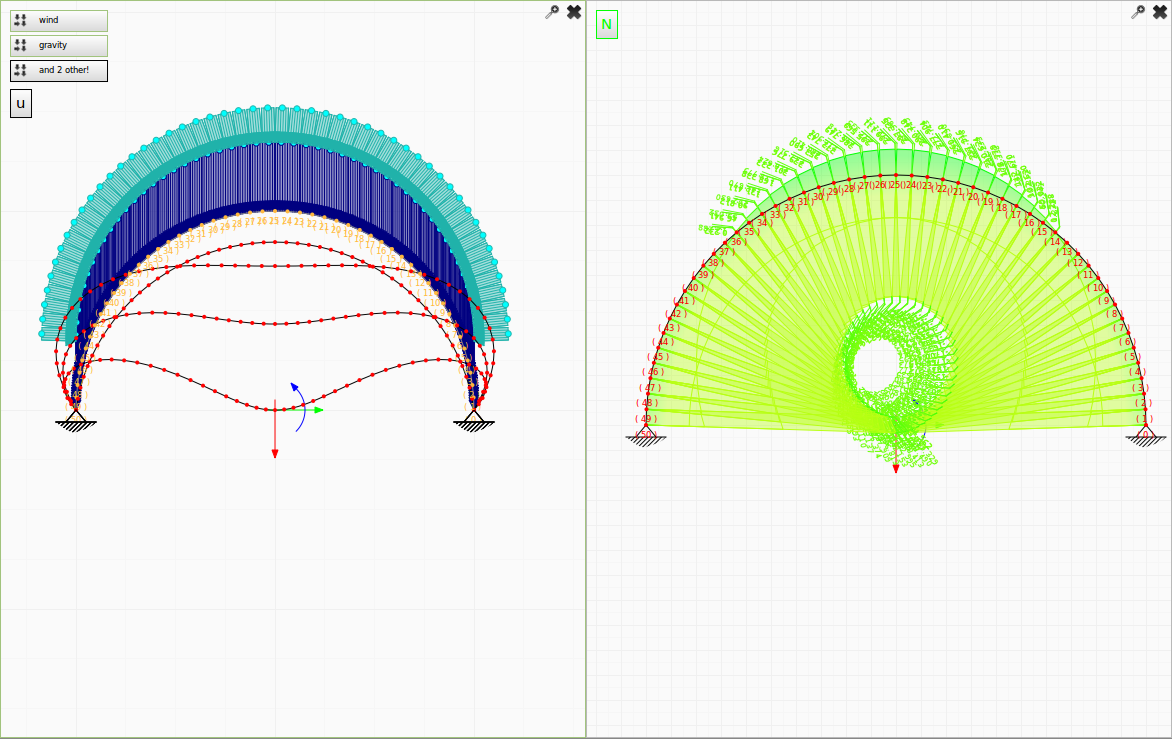
\includegraphics[width=\textwidth]{../pictures/scriptclsfinished.png}
\caption{normal force in the arc for more combinations of loads}
\label{pic:scriptclsfinished}
\end{center}
\end{figure}
\vspace{20pt}\\


\begin{lstlisting}[frame=single, basicstyle=\small, label=lst:setcreation, caption=creating load sets, numbers=left, firstnumber=1, tabsize=3]
//create load sets
struct.addBLS(ColinBLS("gravity"));
struct.addBLS(ColinBLS("wind"));
struct.addCLS(ColinCLS("wind"));
struct.addCLS(ColinCLS("gravity"));
struct.addCLS(ColinCLS("wind+gravity"));
struct.addCLS(ColinCLS("wind+gravity2"));
for(i=0; i<struct.loadCount; i++){
	load = struct.getLoad(i);
	load.set=0;
	struct.setLoad(i, load);
}
for(i=0; i<struct.beamCount; i++){
struct.addLoad(ColinLoad(2, i, Math.sin(struct.getBeam(i).angle)*500, -Math.cos(struct.getBeam(i).angle)*500, 0, 1));
}
//creating cls with a single bls
struct.addBLStoCLS(/*cls*/0, /*bls*/0, /*factor*/1);
struct.addBLStoCLS(/*cls*/1, /*bls*/1, /*factor*/1);
//creating wind+gravity
wg = struct.getCLS(2);
wg.children = new Array(2);
wg.children[0] = new Object;
wg.children[0].bls = 0;		//gravity
wg.children[0].factor = 1.35;	//*1.35
wg.children[1] = new Object;
wg.children[1].bls = 1;		//wind
wg.children[1].factor = 1.5;	//*1.5
struct.setCLS(2, wg);
//creating wind+gravity2
wg = struct.getCLS(3);
wg.children = new Array(2);
wg.children[0] = new Object;
wg.children[0].bls = 0;		//gravity
wg.children[0].factor = 0.9;	//*0.9
wg.children[1] = new Object;
wg.children[1].bls = 1;		//wind
wg.children[1].factor = -1.5;	//*-1.5
struct.setCLS(3, wg);
\end{lstlisting}
